\chapter{Dati e infrastruttura di ricerca}
\label{ch:dati}

Questo capitolo descrive il contesto istituzionale del mercato su cui opera
la strategia (\S\ref{sec:dati-deribit}), i dataset impiegati
(\S\ref{sec:dati-dataset}) e i tre pilastri metodologici dell'infrastruttura
di ricerca: la stima della volatilità realizzata
(\S\ref{sec:dati-rv}), l'estrazione della densità risk-neutral
(\S\ref{sec:dati-rnd}) e il framework di backtest walk-forward
(\S\ref{sec:dati-backtest}). Chiude con la caratterizzazione dei due periodi
di analisi (\S\ref{sec:dati-contesto}).

\section{Il mercato Deribit}
\label{sec:dati-deribit}

Deribit è la sede di negoziazione dominante per le opzioni su criptovalute,
con una quota superiore all'80\% del volume globale di opzioni Bitcoin. La
concentrazione della liquidità su un'unica piattaforma è una caratteristica
peculiare del mercato crypto e presenta un vantaggio per la ricerca: i
prezzi osservati provengono da un unico order book profondo, senza i
problemi di frammentazione e di consolidamento delle quotazioni tipici dei
mercati azionari multi-venue.

Le opzioni quotate su Deribit sono europee e di tipo \emph{inverse}: il
premio e il regolamento avvengono in Bitcoin, mentre lo strike è denominato
in dollari. Questa struttura ha un'implicazione tecnica rilevante per il
calcolo della volatilità implicita, poiché il payoff espresso in valuta di
base non è lineare nel prezzo del sottostante come nelle opzioni classiche.
La copertura direzionale della strategia utilizza i \emph{futures
trimestrali} anziché i \emph{perpetual}. La scelta è motivata dai costi: i
futures perpetui incorporano un tasso di \emph{funding} che, nei mercati
rialzisti, diventa strutturalmente oneroso per chi detiene posizioni corte,
mentre i futures trimestrali presentano una base fissa e prevedibile, priva
di funding. Deribit pubblica inoltre l'indice DVOL, una misura di
volatilità implicita a 30 giorni costruita con metodologia analoga al VIX,
che nel presente lavoro funge da riferimento per la volatilità implicita di
mercato.

\section{I dataset}
\label{sec:dati-dataset}

L'analisi si fonda su due corpora di dati principali: le opzioni Bitcoin di
Deribit per la strategia e per la validazione in-sample e out-of-sample, e
le opzioni SPY per la validazione cross-asset del
Capitolo~\ref{ch:validazione}. La Tabella~\ref{tab:dataset} ne riassume le
caratteristiche.

\begin{table}[H]
\centering
\caption{Dataset impiegati nell'analisi.}
\label{tab:dataset}
\small
\begin{tabular}{lllc}
\toprule
\textbf{Dato} & \textbf{Fonte} & \textbf{Frequenza} & \textbf{Periodo} \\
\midrule
Opzioni BTC (EOD) & Deribit & giornaliera & giu 2021 -- set 2024 \\
Spot BTC & Deribit & giornaliera & giu 2021 -- set 2024 \\
Perpetual BTC & Deribit & 5 minuti & giu 2021 -- set 2024 \\
Futures trimestrali BTC & Deribit & giornaliera (OHLC) & giu 2021 -- set 2024 \\
Funding rate & Deribit & giornaliera & giu 2021 -- set 2024 \\
Indice DVOL & Deribit & giornaliera & giu 2021 -- set 2024 \\
Opzioni SPY (EOD) & optionsDX & giornaliera & gen 2010 -- dic 2023 \\
\bottomrule
\end{tabular}
\end{table}

I file EOD mensili delle opzioni Bitcoin sono stati consolidati in un unico
dataset per il backtest. I prezzi delle opzioni sono espressi in Bitcoin
(coerentemente con la struttura inverse) e convertiti in dollari al prezzo
spot del giorno dove necessario per il calcolo del profitto e delle
metriche di rischio. Il dataset SPY, impiegato solo per la validazione
cross-asset, comprende file EOD giornalieri per quattordici anni, per un
totale di circa 9,5 milioni di record.

La qualità dei dati è un tema centrale per una strategia che vende opzioni,
poiché le distorsioni nei prezzi di strumenti illiquidi possono generare
profitti fittizi. Due aspetti meritano segnalazione. Primo, sul mercato
Bitcoin le opzioni profondamente in-the-money sono spesso prive di
quotazioni reali: il loro \emph{bid} nei dati risulta pari a zero, non
perché abbiano valore nullo ma perché nessun operatore le quota in
acquisto. Come documentato nel Capitolo~\ref{ch:percorso}, questo dettaglio
è all'origine di un artefatto che ha invalidato una delle strategie
esplorate, e ha motivato l'introduzione di un filtro sul delta. Secondo,
nel dataset SPY tre record su 9,5 milioni presentano volatilità implicita
negativa nei dati sorgente, con impatto trascurabile ($-11$ dollari sul
profitto totale) ma segnalato per completezza.

\section{Stima della volatilità realizzata}
\label{sec:dati-rv}

La quantificazione del premio per il rischio di volatilità richiede una
misura della volatilità effettivamente realizzata dal sottostante, da
confrontare con quella implicita nei prezzi delle opzioni. Come discusso
nel Capitolo~\ref{ch:letteratura}, la tesi adotta lo stimatore di
\citet{parkinson1980extreme}, basato sull'escursione infragiornaliera
high--low anziché sui soli prezzi di chiusura:
%
\begin{equation}
\hat{\sigma}^2_{P} = \frac{1}{4\ln 2}\,\frac{1}{n}\sum_{i=1}^{n}
\left(\ln \frac{H_i}{L_i}\right)^2,
\label{eq:parkinson}
\end{equation}
%
dove $H_i$ e $L_i$ sono rispettivamente il massimo e il minimo del giorno
$i$, e la stima viene annualizzata e calcolata su una finestra mobile di 30
giorni. La scelta è particolarmente appropriata per Bitcoin, negoziato
ininterrottamente 24 ore su 24 e 7 giorni su 7: l'assenza di sessioni di
chiusura elimina i salti overnight che affliggerebbero lo stimatore
close-to-close, e l'informazione contenuta nel range infragiornaliero è
pienamente disponibile e continua. Sotto le ipotesi del modello, lo
stimatore di Parkinson è circa cinque volte più efficiente di quello basato
sulle sole chiusure.

Il confronto tra il DVOL (volatilità implicita) e la volatilità realizzata
di Parkinson a 30 giorni, mostrato nella Figura~\ref{fig:vrp-btc} del
Capitolo~\ref{ch:introduzione}, evidenzia uno spread medio di 16,2 punti
percentuali annualizzati, positivo nel 93\% delle giornate. È questo il
premio che la strategia si propone di catturare.

\section{Estrazione della densità risk-neutral}
\label{sec:dati-rnd}

L'infrastruttura include una pipeline per l'estrazione della densità
risk-neutral (RND) implicita nei prezzi delle opzioni, basata sul risultato
di \citet{breeden1978prices}, secondo cui la RND è proporzionale alla
derivata seconda del prezzo della call rispetto allo strike:
%
\begin{equation}
q(K) = e^{rT}\,\frac{\partial^2 C(K,T)}{\partial K^2}.
\label{eq:breeden}
\end{equation}
%
In pratica, per ogni giornata e per ogni scadenza la pipeline procede in
quattro passi. Primo, costruisce la \emph{smile} di volatilità implicita a
partire dalle opzioni out-of-the-money (più liquide), applicando la
put-call parity per ricucire il ramo delle put con quello delle call.
Secondo, interpola la smile con una spline cubica su una griglia densa di
strike nell'intervallo di moneyness $[0{,}7;\,1{,}3]$. Terzo, converte le
volatilità interpolate in prezzi di call continui e vi adatta una spline di
quarto grado, di cui calcola analiticamente la derivata seconda per
ottenere la RND secondo l'Equazione~\eqref{eq:breeden}. Il tasso privo di
rischio è posto pari a zero, coerentemente con la prassi per gli strumenti
inverse denominati in Bitcoin. Quarto, la densità viene valutata su una
griglia di 200 punti e normalizzata.

Parallelamente, l'infrastruttura stima la densità fisica (sotto la misura
$\mathbb{P}$) tramite kernel density estimation gaussiana sui log-rendimenti
giornalieri, su una finestra mobile di 365 giorni, con bandwidth di
Silverman $h = 1{,}06\,\sigma\,N^{-1/5}$. Il confronto tra le due densità
era alla base di uno dei segnali di selezione esplorati. Come documentato
nel Capitolo~\ref{ch:percorso}, tale segnale si è rivelato privo di potere
predittivo, per ragioni riconducibili alla fragilità del confronto
\emph{pointwise} tra due densità entrambe stimate con errore; la RND resta
tuttavia un utile strumento di contesto e di analisi, e viene impiegata nel
Capitolo~\ref{ch:percorso} anche per il calcolo di skewness e curtosi
implicite tra gli indicatori di regime testati.

La Figura~\ref{fig:rnd-kde} mostra un esempio rappresentativo delle due
densità, estratte con la pipeline descritta per il 15 giugno 2022, nel pieno
del bear market, per la scadenza a 44 giorni: la densità risk-neutral è
spostata verso destra e più dispersa rispetto alla densità fisica stimata
sui rendimenti storici, coerentemente con una volatilità implicita superiore
a quella realizzata.

\begin{figure}[H]
\centering
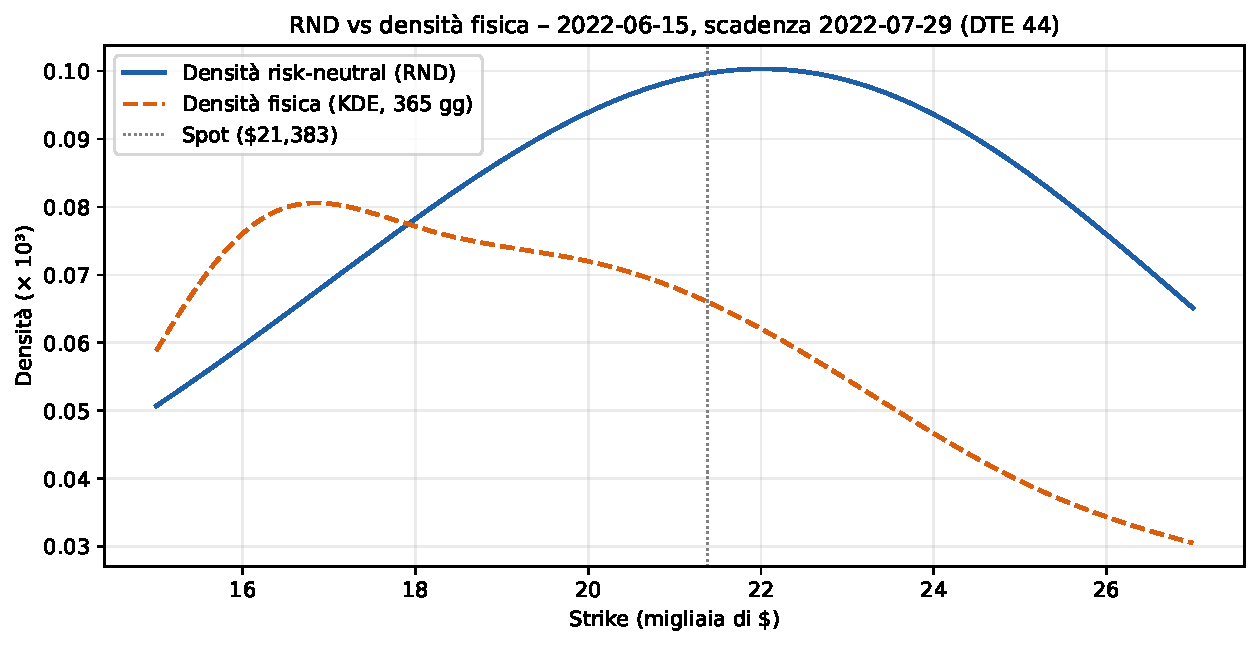
\includegraphics[width=\textwidth]{figures/fig_rnd_kde.pdf}
\caption{Densità risk-neutral (RND, estratta via Breeden--Litzenberger) e
densità fisica (KDE su 365 giorni di rendimenti) per il 15 giugno 2022,
scadenza 29 luglio 2022 (44 giorni). Spot: \$21.383.}
\label{fig:rnd-kde}
\end{figure}

\section{Il framework di backtest walk-forward}
\label{sec:dati-backtest}

Il backtest è organizzato in due fasi, separate per ragioni di efficienza
computazionale. La prima fase, di \emph{scoring}, percorre ogni giornata di
negoziazione, estrae la RND e la densità fisica, e assegna a ciascuna
opzione i punteggi previsti dalla strategia in esame; il suo output è un
file di punteggi precalcolati. La seconda fase, di \emph{simulazione},
legge i punteggi e replica l'attività di trading: selezione dell'opzione,
esecuzione, copertura delta giornaliera, applicazione delle regole di
uscita e imputazione dei costi. La separazione consente di eseguire una
sola volta la parte onerosa (l'estrazione delle densità) e di iterare
rapidamente sulle regole di simulazione.

Due scelte di disegno garantiscono l'assenza di look-ahead bias e il
realismo dei risultati. La prima è la \textbf{tempistica T+1}: il segnale è
calcolato sulla chiusura del giorno $T$, ma l'esecuzione avviene il giorno
$T+1$, al prezzo \emph{bid} dell'opzione (si vende) e al prezzo di apertura
del futures trimestrale. Nessuna informazione del giorno di esecuzione
entra nel segnale. La seconda è la \textbf{valorizzazione mark-to-market
giornaliera}: oltre al profitto realizzato a chiusura di ciascun trade,
l'infrastruttura ricostruisce la curva di equity giorno per giorno,
valorizzando la posizione aperta ai prezzi correnti. Il drawdown calcolato
sulla curva mark-to-market è molto più severo di quello calcolato sui soli
trade chiusi ed è la metrica di rischio primaria adottata in questa tesi,
perché riflette l'esperienza effettiva di chi detiene la posizione.

I costi di transazione sono modellati in modo granulare e conservativo, come
riassunto nella Tabella~\ref{tab:costi}. Le opzioni scontano la commissione
\emph{taker} di Deribit, pari allo 0,03\% del sottostante per lato, con il
tetto regolamentare del 12,5\% del prezzo dell'opzione; lo spread bid-ask è
incorporato direttamente valorizzando l'ingresso al bid e l'uscita all'ask.
La copertura sconta uno 0,10\% per lato, scomposto in commissione (0,05\%),
metà spread (0,03\%) e slippage (0,02\%).

\begin{table}[H]
\centering
\caption{Modello dei costi di transazione.}
\label{tab:costi}
\setlength{\tabcolsep}{4pt}
\begin{tabular}{lll}
\toprule
\textbf{Voce} & \textbf{Costo} & \textbf{Note} \\
\midrule
Commissione opzione & 0,03\% del sottostante / lato & cap al 12,5\% del premio \\
Spread opzione & incorporato & entry al bid, exit all'ask \\
Commissione hedge & 0,05\% / lato & futures trimestrali \\
Mezzo spread hedge & 0,03\% / lato & \\
Slippage hedge & 0,02\% / lato & \\
Funding & assente & scelta dei futures trimestrali \\
\bottomrule
\end{tabular}
\end{table}

L'analisi è condotta con una logica \emph{walk-forward}: i parametri e le
scelte di disegno sono fissati sul periodo in-sample e la loro tenuta è poi
verificata, senza alcuna riottimizzazione, sul periodo out-of-sample. Lo
split temporale, definito una volta per tutte, colloca l'in-sample dal
1\textsuperscript{o} giugno 2021 al 30 settembre 2023 e l'out-of-sample dal
1\textsuperscript{o} ottobre 2023 al 30 settembre 2024.

\section{Contesto di mercato dei due periodi}
\label{sec:dati-contesto}

La scelta dello split non è neutrale rispetto all'interpretazione dei
risultati, perché i due periodi presentano caratteristiche di mercato
profondamente diverse, riassunte nella Tabella~\ref{tab:contesto-mercato}.

\begin{table}[H]
\centering
\caption{Contesto di mercato dei periodi in-sample e out-of-sample.}
\label{tab:contesto-mercato}
\small
\setlength{\tabcolsep}{4pt}
\begin{tabular}{lcc}
\toprule
 & \textbf{In-sample} & \textbf{Out-of-sample} \\
 & giu 2021 -- set 2023 & ott 2023 -- set 2024 \\
\midrule
BTC inizio $\to$ fine & \$36.677 $\to$ \$26.916 ($-27\%$) & \$27.050 $\to$ \$64.543 ($+139\%$) \\
Range di prezzo & \$15.797 -- \$68.368 & \$26.777 -- \$73.285 \\
RV30 media & 57\% & 50\% \\
Carattere & Bear market + range & Bull market \\
 & (crash 2022: $-55\%$ in un trimestre) & (vol in compressione) \\
\bottomrule
\end{tabular}
\end{table}

Il periodo in-sample è il più severo e informativo: comprende il bear
market del 2022, con un trimestre a $-55\%$ per Bitcoin e le tensioni
seguite ai dissesti di operatori del settore. Una strategia short
volatility è strutturalmente esposta proprio agli episodi di questo tipo, in
cui la volatilità esplode e le posizioni corte in opzioni subiscono perdite
mark-to-market immediate. Che la strategia produca uno Sharpe elevato
attraversando questo periodo è dunque il risultato più solido dell'intero
lavoro. Il periodo out-of-sample, al contrario, è un mercato fortemente
rialzista con volatilità in compressione, un contesto favorevole alle
strategie di vendita di volatilità: il suo Sharpe, pur elevato, va letto
con la consapevolezza che le condizioni erano propizie, ed è
verosimilmente sovrastimato rispetto a un regime di mercato neutro. Questa
asimmetria interpretativa tra i due periodi guida la lettura dei risultati
nei capitoli successivi.
